\documentclass[a4paper,10pt, bibliography=totocnumbered]{scrreprt}

\usepackage[utf8x]{inputenc}
\usepackage[english]{babel}

\usepackage{graphicx}
\usepackage{pdfpages}
%\usepackage{subfig}
%\usepackage{microtype}
\usepackage{tabularx}
%\usepackage{amsmath, textcomp}

% Custom packages
\usepackage[numbers]{natbib}
\usepackage{longtable}
\usepackage{ragged2e}
%\usepackage{tikz}
%\usetikzlibrary{positioning}
%\usepackage{pdflscape}
%\usepackage{rotating}

\usepackage{glossaries} 
%Glossar?

\usepackage{hyperref}
\hypersetup{
    colorlinks=true,        % false: boxed links; true: colored links
    linkcolor=black,        % color of internal links
%    citecolor=green,        % color of links to bibliography
    citecolor=black,        % color of links to bibliography
    filecolor=magenta,      % color of file links
    urlcolor=blue           % color of external links
}


%% Title Page
\makeatletter
\renewcommand{\maketitle}{\begin{titlepage}
    \vskip 10\p@
    \hbox{
      \vrule depth 0.99\textheight
        \mbox{\hspace{2em}}
      \vtop{
        \vskip 10\p@
        \hspace{4pt}
        \vskip 50\p@
        \begin{flushleft}
          \Large \@author \par
        \end{flushleft}
        \vskip 50\p@
        \begin{flushleft}
          \huge \bfseries \@title \par
        \end{flushleft}
        \begin{flushleft}
          \Large \bfseries \@subtitle \par
        \end{flushleft}
        \vskip 70\p@
        \begin{flushleft}
          \Large \@publishers \par
        \end{flushleft}
        \vskip 50\p@
        \begin{flushleft}
          \Large \@date \par
        \end{flushleft}
        }}
  \end{titlepage}
}
\makeatother

\author{Jan Kerschbaum}
\title{Opinion Extraction from Forum Posts}
\subtitle{Thema 9} % Was ist damit?
\publishers{\textbf{Advisor University of Heidelberg}\\ Prof. Dr. Barbara Paech, Marcus Seiler}
\date{01. 10., 2022} % MM DD, YYYY Blödes Format



% Deutsche Absaetze:
\parindent 0pt
\parskip 12pt

\textwidth145mm
\setlength{\oddsidemargin}{0.7cm}
\setlength{\topmargin}{-0.5cm}
\setlength{\textheight}{22.5cm}

\begin{document}
\maketitle

\section*{Abstract}
When one produces something, the most relevant metric to that things success will be the customers / users opinion. As such, there has been interest in gathering and understanding these opinions approximately since organised commerce first existed. Modern technology has enabled this like never before, both in terms of sharing, discussing and gathering opinions, as well as in terms of automatically analysing, categorising and presenting them. Nonetheless, ability needs to be followed by a plan to create results. Yet the task of analyzing the large amount of barely-structured data available on customer- and/or user-opinions is a daunting, and seldom attempted, one. As such, we seek here to present and analyze several existing approaches, focusing specifically on the data present in the form of forum posts, in the hope that their methods, and their strengths and weaknesses, may inspire even more effective solutions.
%\end{abstract}

\tableofcontents

\chapter{Introduction}
One of the most important (relatively) directly measurable metrics for most industries will always be what the customers think about the product they do or might want to use. This goes doubly so for any sort of software, as updates can be rolled out to an existing customer base with reasonable difficulty, making repeated updates more realistic. Thus, attaining an understandable and up-to-date overview of users opinions and views on a given product can be invaluable in improving the product and the user experience. This, however, is not so easily attained.\\
In part this comes down to inherent differences in the accessible sources. For this report, we'll be focusing on approaches that employ forum posts as their one and only source, more specifically the programmer-centric site Stack Overflow. Mining opinions from forum posts brings its own set of special circumstances to be accounted for, both useful and hindering. Specifically, forums tend to attract a smaller and more focused group of users than other comparable sources, which tends to means smaller, if still massive, amounts of data, featuring opinions more clustered around the theme of the forum. Further, forums employ a thread-style conversation architecture where each post includes some amount of metadata, from which we can draw as well as the pure text. Nonetheless, the limited accessibility of the data, as well as side-effects like potential forum-specific culture shaping the texts in unexpected ways prove challenging.\\
When it comes to extracting user opinions from even just a limited source set such as forums, the sheer amount of data available and the relative lack of structure has led to various approaches with varying levels of success and varying goals. Opiner\cite {OPINER} and POME\cite{POME} share a common process structure, though the precise methods by which they accomplish each partial task varies. The tools work on the entirety of all answers posted on Stack Overflow, employing the official data dumps, from 2017 and 2014 respectively, in order to avoid API usage limitations, though their approaches could each be applied to the live site in theory. In practice, both implementations begin this process by getting the list of all relevant (that is to say, extant) Java APIs from the Maven central repository, as well as their respective set of otherwise needed data.\\
Opiner uses varies preprocessing techniques to normalise the data, whereas POME applies no such methods. They proceed to detect mentions of individual APIs by comparing the posts to the data they collected about each individual API. The sentences tagged as mentioning specific APIs are then further sorted with regards to the relevant quality aspect, if any, and their sentiment polarity , before the results are stored to a database for later retrieval by the respective online tool (though it is worth mentioning that Opiner sorts by sentiment first, and by quality aspect second, while POME does the opposite. This has no impact in practice as the two sortings are independent from one another). Despite employing this common workflow, however, their methods are quite different.


\chapter{Literature Search}

\section{Research Question}
The second paper examined here was chosen for relevance to both the topic and the provided paper (Opiner \cite{OPINER}). Despite the limited scope of the paper, the research question needed to be oriented towards more open results, as slightly deviating approaches within the same theme could still provide interesting insights. Within these restraints and considerations, the following research question was determined as optimal:
\begin{center}
    "How, and how well, can opinions regarding specific themes be extracted from forum posts?"
\end{center}

\section{Methodology}

A set of criteria was defined to determine whether any given paper was suitable. These included:

\begin{enumerate}
    \item The paper describes an approach for the automatic extraction of opinions from forum posts.
    \item The approach is use-able to extract opinions on multiple themes in a comparable manner.
    \item The paper is less than 10 years old.
    \item The paper must be in English or German.
    \item The paper should be from different authors than the provided paper.
\end{enumerate}

Further, the search term was built from the most important tokens in the question, expanded upon to catch common synonyms.

\begin{center}
    (opinion OR sentiment) AND (extraction OR mining) AND (forum or "Stack Overflow")
\end{center}

Search engines IEEE, ACM and Elsevier were determined suitable for this literature research, on the basis of the paper provided and the criteria.
\pagebreak

\section{Results}

All searches were conducted on the 06. or 07. November 2021, with varying criteria being either implemented immediately into the search or checked manually, depending on what the respective search engine allowed. For example, only on ACM was the ability to limit the search range by date of publication available and employed.

\begin{figure}[!h]
    \centering
    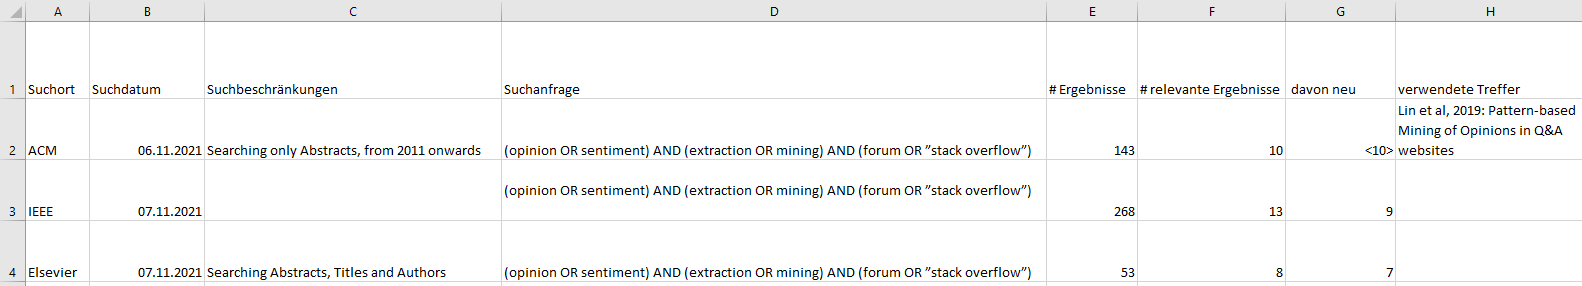
\includegraphics[scale=0.3]{../images/Thema9_Lit.PNG}
    \caption{Literature search results}
    \label{LitSearchResult}
\end{figure}

The initial searches led to varying amounts of results, perhaps owing partially to the different level of conditions implemented immediately upon the search. IEEE proved the most immediately fruitful, with a whole 268 individual results, followed by ACM and Elsevier, providing 143 and 53 results respectively. Of these, only a small portion was relevant, which is defined by fitting all the criteria as well as subjective consideration. (For an example on the latter, a paper discussing an approach that applied to several sources, but did not focus specifically focus on forum posts, was excluded due to the theme, even though it could be considered to satisfy the criteria.)\\
Since the ACM search was the first, all ten of its relevant results were new. The other searches had some overlap in relevant papers found, leaving only nine and seven of their relevant papers, respectively, as new results. These remaining 28 papers were reduced down to a final pool of 8, via a stronger application of the criteria and subjective analysis of abstracts and titles. From those, the paper "Pattern-based Mining of Opinions in Q\&A websites" (Lin et. al., 2019) \cite{OPINER} through full-text relevance comparisons, since it fit the theme well and proposed new and interesting methods, while being reasonably comparable to the approach presented in the provided paper.

\chapter{Approach 1 - Opiner}

\section{Goal}

Opiner \cite{OPINER} seeks to extract and classify sentences from Stack Overflow posts by whether they refer to a specific Java API, and if so which, as well as if any, and if so which, quality aspects of the API are mentioned, in conjunction with the sentences overall sentiment, which is assumed to equal the sentiment of the writer towards that quality aspect of that API.

\section{Algorithm}

After extracting its dataset from the source, Opiner first performs preprocessing in order to normalize the data. The classification task is then split into several steps. First, any given mention of a specific API is detected. Then, it is associated with both a quality aspect and a sentiment. Finally, the data is summarised for easy presentation in the tool.

\subsection{Preprocessing}

Opiner applies relatively standard preprocessing techniques. Specifically, it first removes stop-words, including both standard English stop-words, domain-specific stop-words, as well as country and educational codes. (".com", ".edu", ".de", etc.) Further, each sentence is tokenized and POS-tagged, and sorted into one of four categories; "code terms“, "code snippets“, "hyperlinks“ or "natural language text“. Further use of these categories is not discussed in the paper. 

\subsection{API Mention Detection}

API mentions are detected using a mixture of named-entity an linked-entity detectors. The named-entity detectors search the given sentence for a mention of an APIs full or abbreviated name, while the linked-entity detector checks if any given link connects to online resources for a specific API. If none of these methods returns a clear match, the API mention resolver builds a mention-candidate list (MCL), of reasonable guesses, and the correlates the information from that specific sentence with whats saved in the database about that API, to heuristically determine which of them has the highest chance of being correct. Sentences can also simply not contain a mention of any API. Further, any APIs whose name includes the terms "demo" or "example", or any API that does not have archived source code, is discarded.

\subsection{API Quality Aspect Association}

Through a survey of developers conducted before the paper, a list of 10 relevant quality aspects was determined. (Performance, Useability, Security, Documentation, Compatibility, Portability, Community, Legal, Bug,and those that have a sentiment but aren't related to any quality aspect.) Further, the "other" class was established for sentences that refer to a quality aspect that isn't one of those 10. 4000 example sentences were human-labeled to serve as a gold standard, and a binary classifier for each class was trained on them.

\subsection{Sentiment Analysis}

The specific algorithm by which Opiner conducts its sentiment analysis is not fully discussed in the paper, though it is compared to the preexisting SentiStrength and Sentiment Orientation algorithms. As such, it is likely that is shares a general outline with them, by first tagging all words which independently evoke a sentiment with a value, then applying the effects of booster words that relate to them, before finally collecting the minimum and maximum across the whole sentence. The actual value of the sentiment is discarded, only the polarity is considered.

\subsection{Summarisation}

Since the goal is in part to present the gathered information in a useful manner, the large corpus of analysed data needs to be summarised somewhat. Opiner specifically does this by sorting the sentences by the quality aspect they relate to, and contrasting them by sentiment polarity. Various statistical metrics are calculated on the sentiments. Some sentences are presented in an abstracted manner.

\section{Tool}

Opiner provides an online tool that fully implements and automates its functionality. A user enters the name of the API they are interested in (or enters a quality aspect or usage scenario and chooses from the presented list of relevant APIs), and is presented with the APIs specific page. (See below.) From here, the viewer can access the various summaries previously constructed through the pages tabs. 

\begin{figure}[!h]
    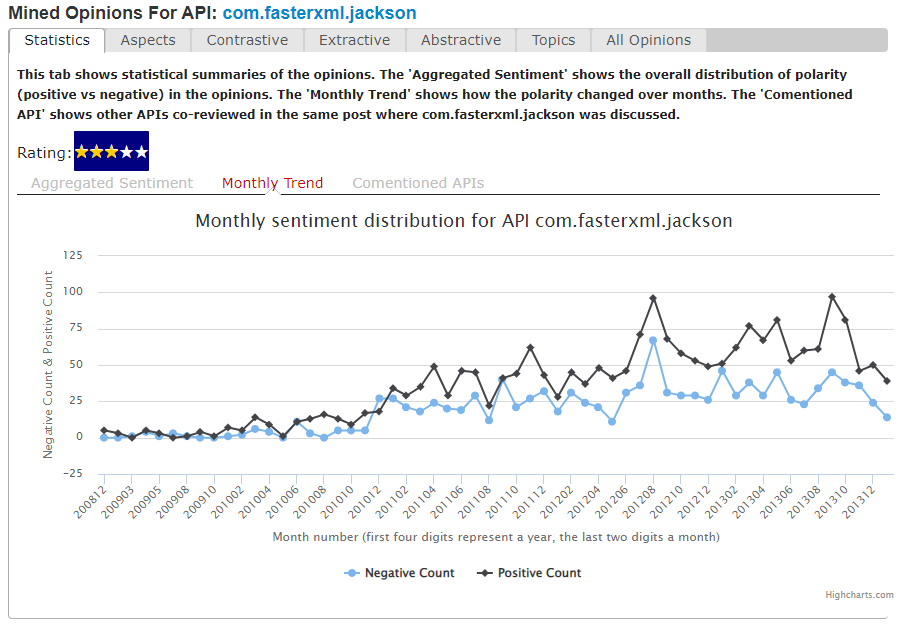
\includegraphics[scale=0.6]{../images/Thema9_OpinerTool0.PNG}
    \caption{Main page for com.fasterxml.jackson (Opiner)}
    \label{OpinerTool0}
\end{figure}

\pagebreak

\section{Evaluation}

To evaluate the effectiveness of Opiner, two binary selection tasks between two APIs each were constructed. Participants were asked to select one of the APIs for a given task, using either Stack Overflow alone or in conjunction with Opiner, and were graded on the correctness of their selection, the confidence with which they made it (self-reported) and the time it took them. The paper does not elaborate on how the correct choice for each task was determined, nor how comparing more than two APIs might affect the results.

\begin{figure}[!h]
    \centering
    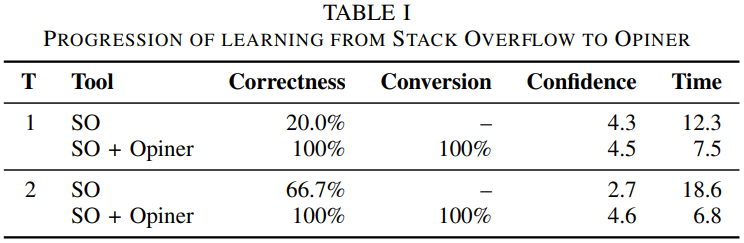
\includegraphics[scale=0.6]{../images/Thema9_OpinerEval.PNG}
    \caption{Evaluation results for Opiner}
    \label{OpinerEval0}
\end{figure}

\subsection{Results}

The correctness of participants choices increased from 20\% and 66.7\% respectively to 100\%. Confidence in task 2, where it was lower to begin with, rose to the same level as in task 1. Time taken was halved for task 1, and cut to almost a third from task two. The inconsistencies in the improvements made by using Opiner were not discussed.

\section{Example}

Consider the sentence "Gson is the fastest library out there." Let's assume this is one of the sentences Opiner mined from Stack Overflow. It first undergoes preprocessing, which might leaves us with a POS-tagged sentence along the lines of "Gson fastest" (Note that the full list of removed stop-words is not reproduced.) Opiner then attempts to detect which API is being mention, and in this case the API Gson is directly named, so we have a clean match. The remaining sentence fragment is the classified by the classifiers as to the relevant quality aspects, and being assigned a sentiment polarity. While the tools used for this aren't publicly available, it seems reasonable to assume this sentence would be assigned a positive sentiment and the quality aspect performance. The sentence is the saved with its list of quality aspects and its sentiment polarity to the database, and once this is done for all sentences for a given API, the summaries are prepared. 

\chapter{Approach 2 - POME}

\section{Goal}

POME \cite{POME} seeks to extract and classify sentences from Stack Overflow posts by whether they refer to a specific Java API, and if so which, as well as if any, and if so which, quality aspects of the API are mentioned, in conjunction with the sentences overall sentiment, which is assumed to equal the sentiment of the writer towards that quality aspect of that API.

\section{Algorithm}

After extracting  its dataset  from the  source, POMEs classification task is split into several  steps. First, any given mention of a specific API is detected. Then, it is associated with both a quality aspect and a sentiment. Finally, the data is summarised for easy presentation in the tool. Notably, no preprocessing is done.

\subsection{Preprocessing}

No preprocessing is applied, as the information that would be removed in the generalization is exploited later on.

\subsection{API Mention Detection}

POME detects API mentions using named-entity detectors implemented through regular expressions. The search a given sentence for a mention of any APIs fully qualified API type (eg. "com.google.code.gson"), unqualified API type (eg. "Gson"), link to the APIs documentation, or a mention of a specific method of a specific class of the API. The latter could produce false positives, as the authors note, though the benefits are considered to outweigh the negatives. POME does not implement any sort of "fuzzy" matching, meaning that only clear API mentions are considered.

\subsection{API Quality Aspect Association \& Sentiment Analysis}

Through subjective analysis of a human-labeled subset of the data, the authors found patterns that coincided with discussion about specific quality aspects and/or sentiments. These patterns were generalised and assigned a specific quality aspect and sentiment to which they were considered to refer. These rules are lexical structures, codifying syntactic or semantic information, that either are or are not matched by a specific sentence. Since sentences may match several rules, they may match sever quality aspects. How a sentence matching several rules with different sentiment polarities is handled is not mentioned by the authors. As the rule shown in figure 4.1, a rule may work on the sentences lexical dependency graph. The authors do not note whether all rules work like this, or whether they may exploit other syntactical or semantic structures.

\begin{figure}[!h]
    \centering
    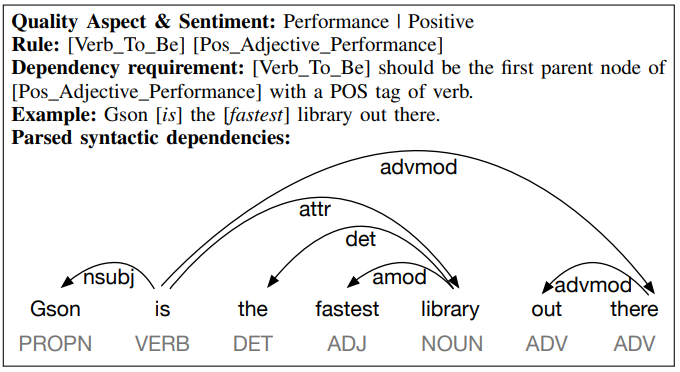
\includegraphics[scale=0.6]{../images/Thema9_Regel.PNG}
    \caption{Rule example}
    \label{POMERule}
\end{figure}

\subsection{Summarisation}

Since the goal is in part to present the gathered information in a useful manner, the large corpus of analysed data needs to be summarised somewhat. POME specifically does this by sorting the sentences by the quality aspect they relate to, and contrasting them by sentiment polarity. Various statistical metrics are calculated on the sentiments. APIs are further directly compared to similar APIs through the statistical metrics.

\section{Tool}

POME provides an online tool that fully implements and automates its functionality, though the paper neglects to link it. No publicly accessible implementation of the tool is known. A user enters the name of the API they are interested in, and is presented with the APIs specific page. (See below.) From here, the viewer can access the various summaries previously constructed through the pages tabs. 

\begin{figure}[!h]
    \centering
    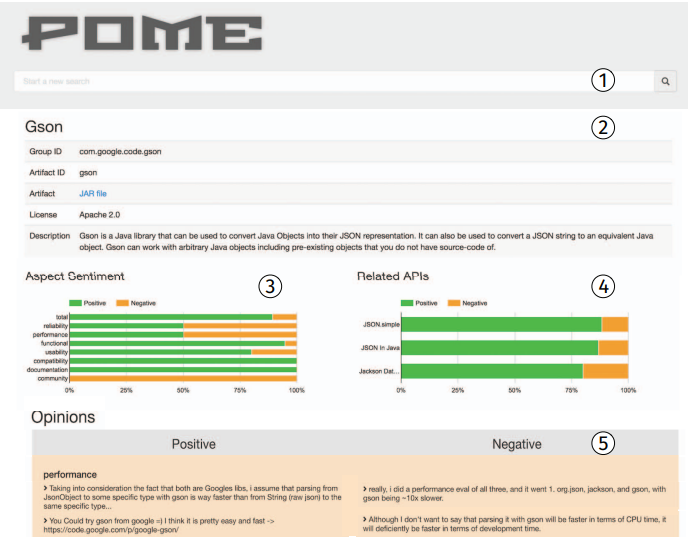
\includegraphics[scale=0.6]{../images/Thema9_POMETool.PNG}
    \caption{POME Tool}
    \label{POMETool}
\end{figure}

\pagebreak

\section{Evaluation}

POMEs evaluation consisted of a total of 3 research questions. RQ 1 and 2 sought to compare the rules-based aspect classifier and sentiment polarity analyzer developed for the paper against their respective state-of-the art equivalents, while RQ 3 compared POME to Opiner in a complete system test. RQ 1 and 2 worked on a subset of 1662 sentences referring to 136 different APIs. For RQ1, the classifier was compared in precision and recall to ML-based classifiers using various feature sets. For RQ2, the sentiment polarity analyzer was compared to various other tools in terms of precision and recall for both positive and negative opinions. For RQ3, 4 APIs were chosen, and the sentences found by POME were human-labeled as a gold standard. The results from both were then gathered through their tools, with the information from Opiner being adjusted to fit POMEs architectural choices, such as the different set of quality aspects, and the lack of fuzzy matching for API mentions. The paper makes no attempts to consider the potential pro-POME bias resulting from this. The two datasets were then compared by their precision in predicting both quality aspects and sentiment polarities, on a per-aspect basis.

\subsection{Results}

POMEs aspect classifier compares favourably to all binary classifier models, only being occasionally beaten by the model that considers the sentences words under BOW, in conjunction with the extant n-grams as well as which patterns were fulfilled. The paper made no attempt to discern whether this was influenced by the patterns being defined on the same dataset from which the test data came, and in the same way no attempt was made to generalise the dataset. Specifically, the fact that the ML-classifiers could never predict, for example, the community aspect, throws the dataset into question.

\begin{figure}[!h]
    \centering
    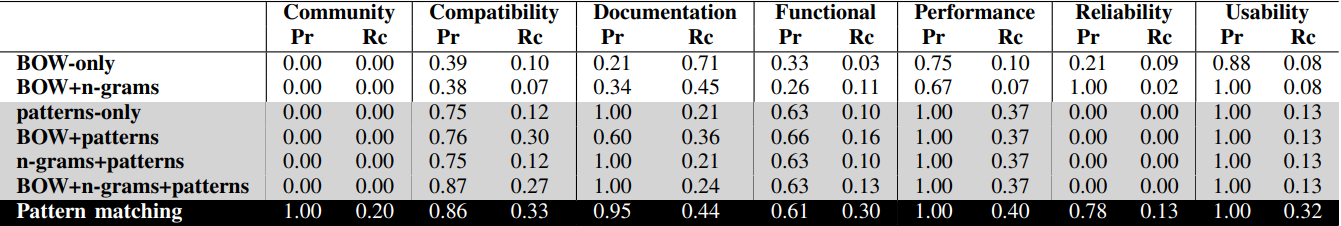
\includegraphics[scale=0.4]{../images/Thema9_POMEEval1.PNG}
    \caption{POME Eval RQ1}
    \label{POMEEval1}
\end{figure}

RQ2 shows similar results to RQ1, with POMEs sentiment analyzer outstripping all but Stanford Core NLP in all metrics, tying with the latter in terms of each being better in two metrics.

\begin{figure}[!h]
    \centering
    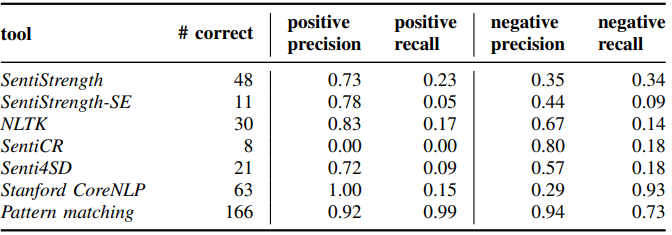
\includegraphics[scale=0.6]{../images/Thema9_POMEEval2.PNG}
    \caption{POME Eval RQ2}
    \label{POMEEval2}
\end{figure}

POME beats Opiner in all metrics quite handily. The sheer difference, especially compared to Opiners much better performance in its own evaluation, makes it questionable how much the theoretical pro-POME bias may rule this result.

\begin{figure}[!h]
    \centering
    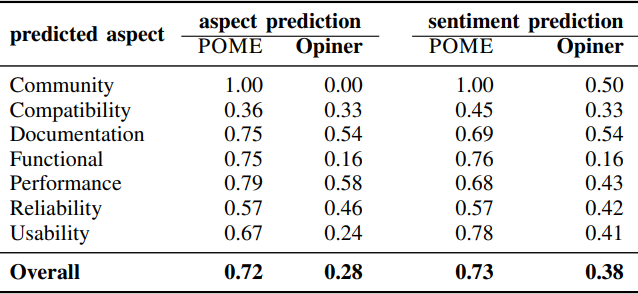
\includegraphics[scale=0.6]{../images/Thema9_POMEEval3.PNG}
    \caption{POME Eval RQ3}
    \label{POMEEval3}
\end{figure}

\section{Example}

Consider the sentence "Gson is the fastest library out there." Let's assume this is one of the sentences Opiner mined from Stack Overflow. This fits the pattern example discussed above, meaning it will be associated with a positive sentiment polarity and the performance quality aspect. Any other matching rules apply similarly, and conflicts are then resolved. The sentence is the saved with its list of quality aspects and its sentiment polarity to the database, and once this is done for all sentences for a given API, the summaries are prepared. 

\chapter{Synthesis}

\section{Methods Employed}

\subsection{Preprocessing}

Opiner applies a relatively wide array of preprocessing techniques both conventional and issue-specific. The removal of stop-words is a common step take to lower the amount of words that need processing, while limiting the impact to the actual relevant data. Opiner expands on this by removing not just standard (English) stop-words, but domain-specific stop words, and country and institutional codes, which come with fully qualified API types, as well. Each sentence is tokenized and POS-tagged for easier processing, after which they're sorted into one of four categories. This sorting isn't mentioned afterwards in the paper, so its full purpose is unclear, though it is likely another preparation to speed up processing later on.\\
POME does not apply preprocessing at all. This is due to its use of lexical patterns, which encode syntactical and semantic information, which would be lost with most common preprocessing steps.\\
The approaches differing use of preprocessing stems from the need of their processing steps. Opiner employs ML-based classifiers, for which it is preferable to have words with similar meaning be treated as the same feature, and where the loss of words with little individual information presents little to no issue. By contrast, the lexical patterns employed by POME would likely largely break, as they rely on syntactic information, which defines the relationship between words, meaning that the loss of any word would carry a risk beyond its individual information. Further, the reliance on semantic information makes other common preprocessing steps such as stemming counterproductive as well, as this information would be fully or partially lost.

\subsection{API Mention Detection}

Opiner detects an API mention by the APIs full or abbreviated name, or by a link to the APIs official resources. Should no clear mention be detected, then Opiner will construct a mention-candidate-list, from which the most likely is selected by heuristically correlating the surrounding meta-information with what is saved about these APIs in the database schema.\\
POME detects API mentions through regular expression-based named-entity detectors. It detects mentions by the fully qualified or unqualified API type, or a link to the APIs official documentation. Further, it allow a specific mention of a specific class to count as an API mention. POME implements no fuzzy matching.\\
Both approaches implement relatively similar mention detection strategies. Where they diverge is mainly in that POME allows an extra category of mentions but does not allow fuzzy matching, opposite to Opiner. POMEs extra category does increase the possibility of false positives, but may help match true mentions in longer conversation where an API is being referred to but not necessarily mentioned repeatedly because the participants are aware of what they are discussing. The difference in whether to implement fuzzy matching is not commented on in either paper, though its absence may help mitigate the false positive rate for POME.

\subsection{API Quality Aspect Association}
Opiner assigns a given sentence one or more of its 10 quality aspects (including one for pure sentiments) through the use of a binary classifier per quality aspect. These were trained on 4000 human-labeled examples. the 'other' class is used as a fallback, if no quality aspect applies.\\
POME analyses to which quality aspects a sentence refer trough its use of lexical patterns. Each of the patterns, formed through largely subjective analysis of the dataset, is identified with a quality aspect to which it indicates a matching sentence is referring to. Since sentences may match several rules, a given sentence may belong to none or as many as all 7 quality aspects.\\
The use of different quality aspects stems from their different sources. Opiners quality aspects were decided upon through a survey of developers, that is to say the intention was to measure what developers think is important about an API. The POME authors, meanwhile decided upon the relevant quality aspects while labeling the sentences that would later be used for analysis, in effect modelling an approximation of what developers actually talk about. Since neither paper explores the implications of this choice, its effects can only be speculated about. Opiners use of binary classifiers promises to be more versatile than POMEs rules, in that it could in theory be applied to other datasets without need for much adjustment. The rules, however, may model the dataset more closely than the transformations learned by the classifier, since a trained professional may notice and exploit nuances and connections that an ML-Algorithm cannot. Conclusive evidence of this is lacking in either paper, however. Lastly, it is worth noting that unlike Opiner, POME makes no note of using a fallback category., rather sorting all sentences into some quality aspect. The implications of this choice, and its potential to form less cohesive quality aspect sentence clusters, is not explored.

\subsection{Sentiment Analysis}

Opiner performs sentiment analysis through a not-fully-specified algorithm, that is noted to take inspiration from the preexisting SentiStrength and Sentiment Orientation Algorithms. While the exacting functioning is thus unclear, it can be inferred that it works by labeling certain words with a sentiment score, and then computing boosters, both pursuant to a dictionary, before gathering sentence-wide maxima and minima. Only the sentiment polarity, as opposed to the exact score, is retained.\\
Much like with the quality aspect association, POME employs its set of rules for this task. Each rule is identified with a sentiment polarity, so a sentences polarity can be constructed from the polarity of the rules they match. The paper neglects to mention whether neutral polarity is possible, or how conflicts (that is, if one sentence matches rule identified with opposite polarities) are handled.\\
Both approaches do not employ any new algorithm here, though in radically different ways. Whereas Opiner employs externally developed tools, which are developed and optimised for application to a wide set of corpuses, POME once again employs the rules it has already used for quality aspect association, which more accurately model the specific dataset. Research Question 2 of POMEs evaluation does seem to indicate that this does perform better on the dataset than more generic tools, but since the applicability to different datasets isn't considered, it's hard, if at all possible, to call either approach 'better' or 'correcter' on this.

\subsection{Summarisation}

Opiner summarises its results by sorting the sentences by the quality aspect they relate to, and contrasting them by sentiment polarity. Various statistical metrics are calculated on the sentiments. Some sentences are presented in an abstracted manner.\\
POME summarises its results by sorting the sentences by the quality aspect they relate to, and contrasting them by sentiment polarity. Various statistical metrics are calculated on the sentiments. APIs are further directly compared to similar APIs through the statistical metrics.\\
The two approaches summarize their respective results in relatively similar manners, which may be due to the similarities in their goal and sources. Nonetheless, in its increased comparative focus between APIs, rather than on simply on API in isolation, POMEs summarisation can be seen as a more advanced version of Opiners.

\section{Classification Goal}

Opiner seeks to extract and classify sentences from Stack Overflow posts by whether they refer to a specific Java API, and if so which, as well as if any, and if so which, quality aspects of the API are mentioned, in conjunction with the sentences overall sentiment, which is assumed to equal the sentiment of the writer towards that quality aspect of that API.\\
POME seeks to extract and classify sentences from Stack Overflow posts by whether they refer to a specific Java API, and if so which, as well as if any, and if so which, quality aspects of the API are mentioned, in conjunction with the sentences overall sentiment, which is assumed to equal the sentiment of the writer towards that quality aspect of that API.\\
The approaches serve the exact same goal, which is part of the  reason they are so readily compared. This is partially caused by POMEs authors taking inspiration from Opiner, and specifically seeking to improve upon it.

\section{Prerequisites and Restrictions}

Opiners infrastructure requires the assumption that all relevant APIs are known from when the approach is first deployed. It also fails to distinguish between different versions of the same API, which is especially questionable when one remembers that matters like the presence of bugs and the useability, both common factors to be improved over an APIs lifespan, are among its quality aspects. Opiner also largely fails to consider potential quality aspects beyond the original, static list.\\
POMEs infrastructure requires the assumption that all relevant APIs are known from when the approach is first deployed. While it distinguishes between different versions of any given API, it does this by outright only ever considering the newest version of any API, which is a transparently flawed strategy. POME also largely fails to consider potential quality aspects beyond the original, static list.

\pagebreak

\section{Supported Development Steps}

Both approaches support developers when selecting (Java) APIs for specifics tasks, and when planning.

\section{Supported Stakeholders}

Both approaches support developers when selecting (Java) APIs for specifics tasks, and further project managers and similar stakeholders on API development projects.

\section{Tools}

Bot approaches implement a tool that executes their process for the user, though only the Opiner tool appears to be online and accessible. The POME-authors neglect to link to their tool.

\section{Level of Automation}

Both tools automate the full process described for the respective approach.

\section{Evaluation}

Opiner was evaluated through a single research question, formulated as both a full system test, and a comparison between the situation before and after the introduction of the tool. This was formulated as a set of two tasks, to be completed by the participants, which include choosing between two APIs for a given task, with or without the tool. These were graded on the correctness of the choice, the confidence the participant had in the choice, as well as time taken. The paper makes no mention of how the correct choice was decided.\\
POME was evaluated through three research questions. The first two compare the rules-based quality aspect classifier and sentiment analyser respectively against state-of-the-art tools in their domain. RQ1 compared the quality aspect analyzer to neural nets using a variety of feature sets. RQ2 compared the sentiment analyzer against various preexisting tools, graded on precision and recall on positive and negative opionions. RQ3 compared POME to Opiner on precision on quality aspect and sentiment polarity prediction. For this, a subset of the data was human-labeled, and their respective classifications were drawn from the tools. The data from Opiner was adjusted to fit POMEs design decisions, including the different list of possible quality aspects, and the limit of using only clear matches that POME would recognise, rather than the fuzzy matching in place in Opiner. The potential for bias introduced here was not considered.\\
The evaluation for Opiner consisted only of a full system test, whereas POME tested specific components. This is largely due to the fact that POME introduced a substantially new method, whereas Opiner used methods previously employed for similar tasks. Both evaluations include unexplored biases that make the robustness of the results somewhat questionable.

\subsection{Results}

For participants in the Opiner study, the correctness of the choices made increased from 20\% and 66.7\% respectively up to 100\%. On average, participants confidence in their choices increased, and the time they took to make them dropped substantially.\\
The aspect classifier examined in RQ1 of Opiner compares favourably to all tested nets. The paper makes no attempt to explore whether this has to do with the fact that the patterns were defined on a specific dataset, or how well they would transfer. The sentiment polarity analysis conducted in RQ2 similarly outperforms all but one compared tool on all metrics, tying with the last in terms of the number of overall metrics won. The results for RQ3 shows POME beating Opiner in all 4 metrics over all quality aspects with an extreme offset. How much the strongly different data format affected this is once again not explored.

\RaggedRight
    \begin{tabular}{ m{3cm} | m{4cm} | m{4cm} }
          & Opiner & POME  \\
         \hline
         Methods Employed & Named-entity / linked-entity detectors \linebreak Sentence-level sentiment analysis \linebreak classifier-based aspect sorting & Named-entity / linked-entity detectors \linebreak rules-based pattern-matching aspect sorting \linebreak ML-based aspect sorting \linebreak Pattern-based polarity analysis\\
         \hline
         Classification goal & Aims to classify opinionated sentences by which API is being referred to, if any; which quality aspects are mentioned; and by the sentiment & Aims to classify opinionated sentences by which API is being referred to, if any; which quality aspects are mentioned; and by the sentiment \\
         \hline
         Prerequisites \& restrictions & Assume all relevant APIs are known at outset \linebreak Does not differentiate different versions of the same API \linebreak Only considers predefined quality aspects & Assume all relevant APIs are known at outset \linebreak Only considers the latest version of any given API \linebreak Only considers predefined quality aspects\\
         \hline
         Supported Development Steps & Java API selection for known task or list of tasks & Java API selection for known task or list of tasks\\ 
         \hline
         Supported Stakeholders & Both external and internal customer benefit from a quicker selection of the most appropriate tools & Both external and internal customer benefit from a quicker selection of the most appropriate tools \\
         \hline
         Supported Tools / Prototypes & Full-process tool available online & Full-process tool created, no link in paper \\
         \hline
         Level of Automation & Tool handles full process automatically & Tool handles full process automatically \\
         \hline
         Evaluation & Comparison study using tool vs not using tool & Partial study of specific methods as well as full-tool study \\
         \hline
         Important Results & Correct selection rate increased from 20\% - 66\% to 100\% & Ideal configuration achieves 61\% - 100\% precision, 13\% - 44\% recall \linebreak Pattern-based sentiment analysis performs better than existing tools
    \end{tabular}

\chapter{Conclusion}

Though these approaches intend to fulfill the same goal by taking the same steps, their methods are quite different indeed. Further, there is no reason to believe the methods employed here are the only viable ones. While the task is solved to a degree by either approach, fulfilling it in the best possible way is still an open question, awaiting both further specific research as well as advancements in relevant fields, which could be re-purposed for this task. In turn, we can draw ideas for other tasks, both similar and dissimilar. In particular, the breadth potential applications for the kind of rules introduced by the POME algorithm and similar structures is hard to imagine, though of course only the future will tell what is truly useful. \\
One thing that's notable about these approaches in their positions as largely pioneering algorithms in this area is their extant and functional implementations. Unlike how early proposals are often characterized, here we find fully functional solutions to the issue at hand. Whether this is due to the nature of the issue, or the immediate usefulness, or any number of other factors is unclear, but it certainly paint an optimistic picture for future research.\\
The wider field of natural language processing is ever-changing, continually adapting to the challenges it finds itself facing. This, of course, brings with it a large amount of intentional and incidental innovation. It is almost certainly only a matter of time until some of it will be applicable to this task. And though this is certainly no reason to become complacent in improving solutions for this and related tasks, it does provide a positive perspective on the intertask-applicability of methods.

%% Bibliography
\bibliographystyle{plainnat}
%\bibliography{literature.bib}%Bibliography file name

\begin{thebibliography}{9}

\bibitem{OPINER} G. Uddin and F. Khomh, "Opiner: An opinion search and summarization engine for APIs," 2017 32nd IEEE/ACM International Conference on Automated Software Engineering (ASE), 2017, pp. 978-983, doi: 10.1109/ASE.2017.8115715.

\bibitem{POME} Bin Lin, Fiorella Zampetti, Gabriele Bavota, Massimiliano Di Penta, and Michele Lanza. 2019. Pattern-based mining of opinions in Q\&A websites. In Proceedings of the 41st International Conference on Software Engineering (ICSE '19). IEEE Press, 548–559. DOI:
\url{https://doi.org/10.1109/ICSE.2019.00066}

\end{thebibliography}

\listoffigures

%\listoftables

\end{document}          

